%%%%%%%%%%%%%%%%%%%%%%%%%%%%%%%%%%%%%%%%%%%%%%%%%%%%%%%%%%%%%%%%%%%%%%%%
%                                                                      %
%     File: Base_Algorithm.tex                                      %
%     Tex Master: Thesis.tex                                           %
%                                                                      %
%     Author: Andre C. Marta                                           %
%     Last modified :  4 Mar 2024                                      %
%                                                                      %
%%%%%%%%%%%%%%%%%%%%%%%%%%%%%%%%%%%%%%%%%%%%%%%%%%%%%%%%%%%%%%%%%%%%%%%%

\chapter{Base iQAQE Algorithm}
\label{chapter:Base Algorithm}

% Something, something, HQCC-project collaboration. I should probably mention this earlier than I do at the moment. (It's just some footnote, right now... I should change this, probably. Although, it is not too important, I guess.)

In this chapter, we present the proposed algorithm, \acrshort{iqaqe}, which interpolates between \acrshort{qaoa} and \acrshort{qemc}. We begin with a comparison of the two algorithms, followed by a detailed description of \acrshort{iqaqe}, its theoretical framework, motivation, and workflow.

\section{Comparison of QAOA and QEMC}
To motivate the development of our new algorithm, \acrshort{iqaqe}, we summarize the merits and drawbacks of both \acrshort{qaoa} and \acrshort{qemc}. \acrshort{qemc} has several advantages over \acrshort{qaoa}, including significantly lower qubit requirements ($n = \log_2(N)$ vs. $N$) and the ability to support shallower circuit depths \cite{tenecohen2023variational}. The threshold probability encoding scheme allows \acrshort{qemc} to associate each graph partition with a volume of quantum states, potentially enhancing noise resilience. Moreover, \acrshort{qemc} might be better trainable \cite{tenecohen2023variational}. However, \acrshort{qemc} requires the entire probability distribution at each optimization step to compute the cost, increasing the number of needed shots compared to \acrshort{qaoa}, which only requires expectation values. Additionally, it has been shown that \acrshort{qemc} can be efficiently simulated classically, somewhat undermining its purpose as a quantum algorithm \cite{tenecohen2023variational}.

With a thorough grasp of these two algorithms, the \textit{HQCC}-project collaboration has put forward a novel hybrid algorithm that integrates aspects from both, intending to capitalize on their individual strengths for a more substantial outcome. This is what we will be discussing next.

%%%%%%%%%%%%%%%%%%%%%%%%%%%%%%%%%%%%%%%%%%%%%%%%%%%%%%%%%%%%%%%%%%%%%%%%
\section{Interpolated QAOA/QEMC Hybrid Algorithm (iQAQE)}
\label{section:iQAQE}

% I'll keep the cardinality in [1, 2**(n-1)], for n qubits, under the argument that: 1 - QEMC, and 2**(n-1) - QAOA. Later, I might mention that we relax this constraint, allowing for 2**n - 1, as well. That is only towards the end, when I'm doing those bar plots with performance bins, etc. [Many colours, etc.]

\subsection{Theoretical Framework}
\label{subsection:iQAQE Theoretical Framework}
The proposed algorithm aspires to act as an interpolation between \acrshort{qaoa} and \acrshort{qemc}, aiming to amalgamate the strengths of both into a more robust approach, tentatively named \acrshort{iqaqe} (Interpolated QAOA/QEMC). In \acrshort{iqaqe}, we depart from the \acrshort{qemc} approach by associating each graph node with a list of basis states, in contrast to \acrshort{qemc}'s consideration of a single basis state for each node (cf. Figure \ref{fig:iQAQE_Encoding}). Each of these lists comprises somewhere between $\left[1, 2^{\texttt{n\_qubits}-1}\right]$ basis states, where \texttt{n\_qubits} represents the number of qubits. This design allows for potential overlap among states from different lists/nodes. Additionally, it is important to note that the encoding of these states will utilize a qubit range expected to fall between the \acrshort{qemc} and \acrshort{qaoa} requirements, specifically in $[\log_2{N}, N]$, for an $N$-node graph. With all that said, the main goal of my thesis is to ascertain the optimal mapping from basis states to lists, essentially determining which basis states should be included in specific lists/nodes. Naturally, this undertaking also involves the identification of a suitable cost function and ansatz to ensure the algorithm's effective operation. For most of our work, we consider \acrshort{iqaqe} to use the same ansatz and cost function as \acrshort{qemc}, adjusted for the appropriate number of qubits and with some modifications that we'll discuss below.

% Figure: iQAQE Encoding
\begin{figure}[H]
    \centering
    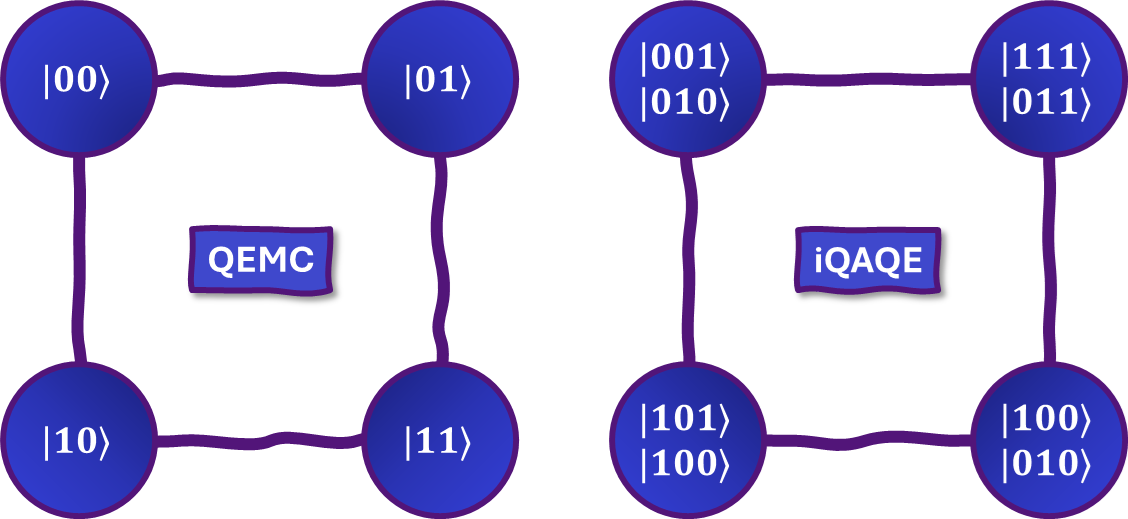
\includegraphics[width=0.8\textwidth]{Figures/Diagrams/QEMC_iQAQE_Encodings.png}
    \caption{Sample schematic representation of the \acrshort{iqaqe} encoding scheme. Comparison between the \acrshort{qemc} and \acrshort{iqaqe} encoding schemes: example for a trivial $4$-node graph. In \acrshort{qemc}, each node is associated with a single basis state, while in \acrshort{iqaqe}, each node is associated with a list of basis states.}
\label{fig:iQAQE_Encoding}
\end{figure}

\subsection{Motivation \& Outlook}
\label{subsection:iQAQE Motivation}
At this point, it is important to mention that the development of this algorithm is entirely exploratory, although we do believe it should allow for a more practical algorithm implementation-wise. We can postulate that such an hybrid approach might have some potential advantages. Namely, it should allow for less shots than in \acrshort{qemc} and fewer qubit requirements than in \acrshort{qaoa}, in addition to, arguably, being better trainable. Another interesting characteristic of such an algorithm is its tunable "quantum-ness". As we interpolate between \acrshort{qaoa} (hybrid quantum-classical) and \acrshort{qemc} (classical, quantum-inspired), the ability to selectively adjust the degree of both could prove to be advantageous. As part of a more long-term perspective (not in this thesis), I may explore the possibility of generalizing this algorithm to tackle additional combinatorial problems, such as Max-$k$-Cut. Throughout my thesis, I will rigorously test the algorithm using classical simulations of quantum machines. The aim is to identify the most effective implementation strategies, taking into account both cost and ansatz considerations, as well as the distribution of basis states.

\subsection{Algorithm Description \& Workflow}
\label{subsection:iQAQE Description_Workflow}
A sketch of the workflow is provided below (Table \ref{tab:iQAQE_Steps}). Following this, I will elaborate on each step. Regarding the hybrid loop, I will only detail the changes relative to \acrshort{qemc}.
\begin{table}[h!]
    \centering
    \begin{tabular}{|c|p{9.5cm}|}
    \hline
    \textbf{Step} & \textbf{Description} \\ \hline
    $1.$ \textbf{Select number of qubits} & \texttt{n\_qubits}$ = n \in \left[\log_2{(N)}, N\right]$, where $N$ refers to the graph's number of nodes. \\ \hline
    $2.$ \textbf{Select list cardinality} & \texttt{list\_cardinality}$ = c \in \left[1, 2^{n - 1}\right]$, where $n$ represents the chosen number of qubits. Note that $c$ is taken to be the same for all the nodes, although this could change in future work. \\ \hline
    $3.$ \textbf{Assignment/mapping} & Map $c$ basis states to each graph node. \\ \hline
    \makecell{$4.$ \textbf{Calculate nodes' probabilities} \\ \textbf{(within the hybrid loop)}} & To obtain each node's probability, sum the probabilities of the basis states in the list and normalize the results, so they add to $1$. \\ \hline
    \makecell{$5.$ \textbf{Cost function and ansatz} \\ \textbf{(within the hybrid loop)}} & Keep the same cost function and ansatz as in the \acrshort{qemc} algorithm, just adapt the ansatz to the correct number of qubits. \\ \hline
    \end{tabular}
    \caption{Steps for the Base-\acrshort{iqaqe} algorithm.}
    \label{tab:iQAQE_Steps}
\end{table}

\subsubsection*{$1.$ Select the number of qubits}
In selecting the number of qubits, we allow for any intermediate value between the \acrshort{qemc} ($\log_2{(N)}$) and \acrshort{qaoa} ($N$) limits. This should give us more flexibility regarding the degree of "quantum-ness" that we want our algorithm to exhibit. This is to be understood in the context of \acrshort{qemc} being entirely classical, whereas \acrshort{qaoa} is hybrid quantum-classical. As such, by choosing a number of qubits in between these two limits, we expect our algorithm to be hybrid in terms of its quantum nature. In addition to this, the number of qubits, alongside the ansatz, will also influence the expressivity of the model.

Another key consideration, closely tied to our next workflow step, is the chosen encoding method. This refers to how we determine each node's color and map basis states to respective lists. Different encoding strategies, such as using expectation values of Pauli strings (e.g., as seen in \cite{sciorilli2024largescale}), inherently influence the number of required qubits. For instance, the Pauli string encoding in \cite{sciorilli2024largescale} automatically enforces a polynomial compression on the number of qubits. Currently, we've employed \acrshort{qemc}'s probability threshold encoding scheme, offering flexibility in deriving node probabilities from basis states. Further discussion on this will be provided in point $4.$ below.

\subsubsection*{$2.$ Select list cardinality}
If it hasn't been clear already, we assign a list of basis states to each graph node. The cardinality of each list, denoted as $c$, falls within the interval $\left[1, 2^{n-1}\right]$, where $n$ represents the number of qubits used. This choice represents a balance between the \acrshort{qemc} ($1$) and \acrshort{qaoa} ($2^{n-1}$) extremes. Determining the optimal value for $c$ is non-trivial, as it depends on various interconnected factors including the number of qubits, ansatz, cost function, and color encoding. To explore its impact on algorithm performance, we conduct grid searches on this parameter.

\subsubsection*{$3.$ Assignments/mapping}
The process of mapping basis states to lists adds significant complexity. \textit{A priori}, there's no clear-cut method for this mapping. The simplest approach involves randomly assigning $c$ basis states to each node, ensuring all states are utilized at least once to avoid discarding information. However, exploring more intricate mappings may yield potential benefits. For instance, in the \acrshort{qaoa} mapping, a single qubit among $N$ is fixed to $1$ for each node, allowing for $2^{N-1}$ permutations of the remaining qubits. Reiterating, each list, comprising $2^{N-1}$ elements, corresponds to a distinct graph node, with each node having a different qubit fixed to $1$. This will result in a myriad of distinct mappings, which we'll thoroughly examine in Chapter \ref{chapter:Schemes_and_Results}, each presenting its unique advantages and disadvantages. The challenge lies in identifying the most effective mapping for a given problem instance. We aim to address this in our work.

\subsubsection*{$4.$ Calculate nodes' probabilities}
Above (Table \ref{tab:iQAQE_Steps}), we mentioned a straightforward method of computing node probabilities by summing the probabilities of associated basis states and normalizing the result. This approach serves as our foundational strategy throughout this work. However, there may be hidden advantages in devising more intricate methods. For instance, one could explore calculating node probabilities using the arithmetic or geometric averages of basis states' probabilities, followed by normalization. Yet, designing such schemes requires caution, as mismatches between the ansatz and encoding could result in constant probabilities for nodes, impeding variational circuit optimization\footnote{This occurred once during testing when we used the \acrshort{qaoa} mapping and ansatz alongside the \acrshort{qemc} cost function and probability threshold encoding scheme.}. Furthermore, the normalization process itself may eliminate the probabilities' dependence on variational parameters under certain circumstances. While we explore alternative methods for calculating probabilities, our primary emphasis in this work remains on the basic approach described earlier, given its apparent robustness.

\subsubsection*{$5.$ Cost function and ansatz}
We employ the \acrshort{qemc} cost function, utilizing the probability threshold encoding scheme mentioned earlier. It's important to note that this scheme assumes, by default, that one of the sets ("Set 1") comprises $B$ nodes\footnote{This value is user-defined.}, which may not align with the MaxCut partition. In some cases, we may need to iterate through potential values of $B$, ranging from 1 to $\left\lfloor{\frac{N}{2}}\right\rfloor$ – although, in practice, careful selection of $B$ should prevent this scenario. Often, setting $B = N/2$ proves to be a reasonable starting point, and we adopt this as our default.

Given our approach to mapping basis states to node lists, it's logical for us to employ the \acrshort{qemc} cost function rather than \acrshort{qaoa}'s. The latter relies on a problem Hamiltonian defined on $N$ qubits, which may not align with our choice of $n$. Typically, $n < N$ as we aim to reduce the number of qubits, making $n = N$ impractical.

Similarly, we opt for the "Strongly Entangling Layers" ansatz from the \acrshort{qemc} scheme for its versatility regarding qubit count. This ansatz, agnostic to specific problems, offers flexibility in our algorithm's implementation compared to \acrshort{qaoa}'s problem-inspired ansatz. However, there are plans to explore more tailored ansatz designs correlated with individual mappings, aiming to enhance algorithm performance by leveraging formulation-specific information. Note that this may necessitate an adjusted objective function developed with these considerations in mind. While we experiment with problem-inspired ansatzë in this work, our primary focus remains on the Strongly Entangling Layers ansatz.

% One of our goals should've been to reduce the number of shots required. However, as it stands, today, we didn't work through that. We've always been doing analytical simulations... At some point in the future, it'd be interesting to explore this further.

% Tomorrow, 14/05, I should go over all this section! Re-read everything and possibly shorten some of this. There will, for sure, be things that I want to remove/change, e.g.

% Describe iQAQE - Explain how it works, its advantages and disadvantages, and its potential applications. Also, mention how iQAQE has many degrees of freedom that can be tuned, which led to the development of many variations of iQAQE, springing from the original idea. These will be described in the \nameref{chapter:Schemes_and_Results} chapter.

% In the PIC2 report, I sort of contradict myself in the end when I mention that "[...] it is somewhat inefficient to iterate over the possible $B$ values [...]". I should correct this (just remove this sentence).

% Sub-lists' cardinalities interval: $[1, 2^N -1]$. In the PIC2 report, it states $[1, 2^{N -1}]$, which is, indeed, what I used for the simulations. However, there's no reason why we shouldn't be allowed to consider $2^N -1$ maximum number of basis states per list. I should put this disclaimer somewhere in here (Thesis).

% In the "Motivation behind this work" section in the PIC2 report, there's a number of things that need to be re-written, before being included here! Remember to do this! (Inefficient $B$ iterations, better trainability - fewer parameters?, etc.)

% There's also a bit of redundancy in this chapter.